% !TeX program = xelatex
\documentclass[12pt,spanish,letterpaper,oneside]{article}
\PassOptionsToPackage{es-noshorthands}{babel}
\def\documenttitle{Señalización de la Muerte Celular Programada}
\def\documentsubtitle{Apoptosis Mediada por el Eje Receptor-Ligando Fas/FasL}
\def\documentsubject{Biología Celular --- Ingeniero Agrónomo}
\def\documentauthor{Diego de la Cruz}
\def\coursename{Biología celular}
\def\coursecode{}
\def\universityname{Universidad Autónoma de Nuevo León}
\def\universityfaculty{Facultad de Agronomía}
\def\universitydepartment{Ingeniero Agrónomo}
\def\universitydepartmentimage{departamentos/logos-institucionales.pdf}
\def\universitydepartmentimagecfg{height=2.1cm}
\def\universitylocation{General Escobedo, Nuevo León, México}
\def\authortable{%
	\begin{tabular}{@{}ll@{}}
		\textbf{Estudiante:} & Diego de la Cruz\\[0.35cm]
		\textbf{Docente Titular:} & Dr. Miguel Ángel Dector Carrillo\\[0.35cm]
		\textbf{Unidad de Aprendizaje:} & Biología Celular\\[0.35cm]
		\textbf{Ponderación Curricular:} & Fase 4: Comunicación y Señalización Celular\\[0.35cm]
		\multicolumn{2}{l}{Fecha de entrega: 15 de noviembre de 2026}\\[0.2cm]
		\multicolumn{2}{l}{\universitylocation}
	\end{tabular}
}

\usepackage{fontspec}
\setmainfont{Arial}
\setsansfont{Arial}
\AddToHook{file/config.tex/after}[aulatex-biologia-celular]{%
  \def\documentfontsize{12}
  \def\documentinterline{1}
  \def\documentparindent{0}
  \def\documentparskip{5}
  \def\fontdocument{custom}
  \def\fonttypewriter{custom}
  \def\stylecitereferences{custom}
  \def\portraitstyle{style1}
  \def\hfstyle{style1}
  \def\hfwidthwrap{true}
  \def\hfwidthtitle{0.44}
  \def\hfwidthcourse{0.52}
  \def\predocpageromannumber{false}
  \def\pagemarginleft{2.5}
  \def\pagemarginright{2.5}
  \def\pagemargintop{2.5}
  \def\pagemarginbottom{2.5}
  \def\firstpagemargintop{3.8}
  \def\sectionfontsize{\large}
  \def\sectionspacingtop{8}
  \def\sectionspacingbottom{4}
  \def\ssectionfontsize{\normalsize}
  \def\ssectionspacingtop{6}
  \def\ssectionspacingbottom{3}
  \def\defaultimagefolder{UANL/ingeniero-agronomo/biologia-celular/img/}
  \def\usepdfmetadata{false}
}
% Template:     Informe LaTeX
% Documento:    Núcleo del template
% Versión:      DEV
% Codificación: UTF-8
%
% Autor: Pablo Pizarro R.
%        pablo@ppizarror.com
%
% Manual template: [https://latex.ppizarror.com/informe]
% Licencia MIT:    [https://opensource.org/licenses/MIT]

% -----------------------------------------------------------------------------
% CONFIGURACIONES
% -----------------------------------------------------------------------------
% Definiciones previas
\input{src/defs}

% Ajustes usuario
\input{src/config}

% -----------------------------------------------------------------------------
% IMPORTACIÓN DE LIBRERÍAS
% -----------------------------------------------------------------------------
\input{src/env/imports}

% -----------------------------------------------------------------------------
% IMPORTACIÓN DE FUNCIONES Y ENTORNOS
% -----------------------------------------------------------------------------
\input{src/cmd/core}
\input{src/cmd/math}
\input{src/cmd/equation}
\input{src/cmd/image}
\input{src/cmd/title}
\input{src/cmd/other}
\input{src/cmd/column}
\input{src/env/environments}

% -----------------------------------------------------------------------------
% IMPORTACIÓN DE ESTILOS
% -----------------------------------------------------------------------------
\input{src/style/code}
\input{src/style/other}

% -----------------------------------------------------------------------------
% CONFIGURACIÓN INICIAL DEL DOCUMENTO
% -----------------------------------------------------------------------------
\input{src/cfg/init}

% -----------------------------------------------------------------------------
% PORTADA
% -----------------------------------------------------------------------------
\input{src/page/portrait}
\input{src/page/portrait_config}

% -----------------------------------------------------------------------------
% CONFIGURACIÓN DE PÁGINA Y ENCABEZADOS
% -----------------------------------------------------------------------------
\input{src/cfg/page}

% -----------------------------------------------------------------------------
% TABLA DE CONTENIDOS - ÍNDICE
% -----------------------------------------------------------------------------
\input{src/page/index}

% -----------------------------------------------------------------------------
% CONFIGURACIONES FINALES
% -----------------------------------------------------------------------------
\input{src/cfg/final}

\RemoveFromHook{file/config.tex/after}[aulatex-biologia-celular]

% -----------------------------------------------------------------------------
% Control de composición anti-huecos, paginación de cierres (Conclusiones y
% Referencias en página nueva independiente) y entorno reutilizable AulatexTable
% (modo encapsulado [\linewidth] y modo multipágina [breakable] con xltabular).
% Requisito editorial del usuario (alcance: materia biologia-celular / carrera).
% -----------------------------------------------------------------------------
\hfuzz=0.5pt
\vfuzz=0.5pt
\renewcommand{\topfraction}{0.90}
\renewcommand{\bottomfraction}{0.85}
\renewcommand{\textfraction}{0.07}
\renewcommand{\floatpagefraction}{0.85}
\renewcommand{\dbltopfraction}{0.90}
\renewcommand{\dblfloatpagefraction}{0.85}
\setcounter{topnumber}{3}
\setcounter{bottomnumber}{2}
\setcounter{totalnumber}{4}
\widowpenalty=10000
\clubpenalty=10000
\raggedbottom

\RequirePackage{etoolbox}
\RequirePackage{placeins}
\RequirePackage{needspace}
\RequirePackage{array}
\RequirePackage{ragged2e}
\RequirePackage{tabularx}
\RequirePackage{longtable}
\RequirePackage{xltabular}
\RequirePackage{booktabs}
\RequirePackage{adjustbox}

\ExplSyntaxOn
\cs_if_exist:NF \aulatexCheckSectionPagebreak
  {
    \cs_new_protected:Npn \aulatexCheckSectionPagebreak #1
      {
        \exp_args:Nnx \regex_match:nnTF { (?i) \A \s* conclusi } { \tl_to_str:n {#1} }
          { \clearpage }
          { \FloatBarrier \needspace{5\baselineskip} }
      }
  }
\ExplSyntaxOff

\makeatletter
\TX@delta=0.5pt
\@ifundefined{NC@rewrite@Z}{%
  \newcolumntype{Z}{>{\raggedright\let\newline\\\arraybackslash\hspace{0pt}}X}%
}{}
\@ifundefined{ifaulatexbreakabletable}{\newif\ifaulatexbreakabletable}{}
\@ifundefined{aulatextablewidth}{\newlength{\aulatextablewidth}}{}
\@ifundefined{AulatexTable}{%
  \newenvironment{AulatexTable}[1][\linewidth]{%
    \par\addvspace{0.20cm}%
    \setlength{\emergencystretch}{2em}%
    \TX@delta=0.5pt%
    \ifstrequal{#1}{breakable}{%
      \aulatexbreakabletabletrue%
      \setlength{\aulatextablewidth}{\linewidth}%
      \setlength{\linewidth}{\aulatextablewidth}%
      \setlength{\hsize}{\aulatextablewidth}%
      \setlength{\LTleft}{0pt}%
      \setlength{\LTright}{\fill}%
      \setlength{\LTcapwidth}{\linewidth}%
      \setlength{\LTpre}{0.15cm}%
      \setlength{\LTpost}{0.15cm}%
    }{%
      \aulatexbreakabletablefalse%
      \setlength{\aulatextablewidth}{#1}%
      \centering%
      \adjustbox{max width=\aulatextablewidth,center}\bgroup%
      \setlength{\linewidth}{\aulatextablewidth}%
      \setlength{\hsize}{\aulatextablewidth}%
    }%
  }{%
    \ifaulatexbreakabletable%
      \par\addvspace{0.20cm}%
    \else%
      \egroup\par\addvspace{0.20cm}%
    \fi%
  }%
}{}

\pretocmd{\subsection}{\needspace{4\baselineskip}}{}{}

\AtBeginDocument{%
  \@ifundefined{aulatexSectionHookInstalled}{%
    \gdef\aulatexSectionHookInstalled{1}%
    \NewCommandCopy{\aulatexOrigSection}{\section}%
    \RenewDocumentCommand{\section}{s o m}{%
      \aulatexCheckSectionPagebreak{#3}%
      \IfBooleanTF{#1}{%
        \aulatexOrigSection*{#3}%
      }{%
        \IfValueTF{#2}{%
          \aulatexOrigSection[#2]{#3}%
        }{%
          \aulatexOrigSection{#3}%
        }%
      }%
    }%
    \@ifundefined{printbibliography}{}{%
      \preto{\printbibliography}{\clearpage}%
    }%
    \BeforeBeginEnvironment{thebibliography}{\clearpage}%
  }{}%
}
\makeatother

% -----------------------------------------------------------------------------
% Marca de Agua Institucional en Portada para Ingeniero Agrónomo (Facultad de Agronomía UANL)
% Recurso de mayor resolución oficial disponible: UANL/assets-uanl/logo-agronomia.png (313x300px RGBA)
% -----------------------------------------------------------------------------
\RequirePackage{eso-pic}
\providecommand{\careerwatermarkimage}{UANL/assets-uanl/logo-agronomia.png}
\providecommand{\institutionalWatermark}[2][0.08]{%
  \AddToShipoutPictureBG*{%
    \put(0,0){%
      \parbox[b][\paperheight]{\paperwidth}{%
        \vfill
        \centering
        \begin{tikzpicture}[remember picture,overlay]
          \node[opacity=#1,inner sep=0pt] at (current page.center) {%
            \includegraphics[width=0.56\paperwidth]{#2}%
          };
        \end{tikzpicture}%
        \vfill
      }%
    }%
  }%
}

\usepackage{microtype}
\usepackage{enumitem}
\usepackage{csquotes}
\usepackage{graphicx}
\usepackage{amsmath,amssymb}
\usepackage[backend=biber,style=apa,sorting=nyt]{biblatex}
\usepackage{tikz}
\usetikzlibrary{positioning,arrows.meta,shapes.geometric}
\definecolor{uanlblue}{RGB}{0,55,108}
\definecolor{tableblue}{RGB}{233,240,247}
\def\portraittitlecolor{uanlblue}
\def\sectioncolor{uanlblue}
\def\ssectioncolor{uanlblue}
\def\documenttitlehf{Muerte Celular Programada (Fas/FasL)}
\fancyfoot[L]{\small \textit{\documenttitlehf}}
\fancyfoot[R]{\small \textit{\coursename}}
\hypersetup{
	colorlinks=true,
	linkcolor=uanlblue,
	urlcolor=uanlblue,
	citecolor=uanlblue,
	pdfauthor={Diego de la Cruz},
	pdftitle={Señalización de la Muerte Celular Programada: Eje Fas/FasL},
	pdfsubject={Biología Celular --- Facultad de Agronomía UANL}
}
\addbibresource{UANL/ingeniero-agronomo/biologia-celular/biologia-celular.bib}

% Control estricto de tipografía y prevención de Overfull/Underfull \hbox
\setlength{\emergencystretch}{3em}
\tolerance=2000
\hbadness=2000
\newcommand{\optsep}{\unskip\hspace{0.55em}\textbar\allowbreak\hspace{0.55em}\ignorespaces}
\newcommand{\selnum}[1]{\textbf{\large\textcircled{\normalsize\bfseries\color{uanlblue}#1}}}

\begin{document}
\hypersetup{pageanchor=false}
% Marca de agua de portada para Ingeniero Agrónomo: Escudo oficial Facultad de Agronomía UANL
\institutionalWatermark[0.08]{UANL/assets-uanl/logo-agronomia.png}
\templatePortrait
\clearpage
\hypersetup{pageanchor=true}
\templatePagecfg
\fancyfoot[L]{\small \textit{\documenttitlehf}}
\fancyfoot[R]{\small \textit{\coursename}}
\singlespacing

\section*{Resumen}
En este reporte técnico se analiza la vía extrínseca de la apoptosis mediada por el complejo receptor-ligando Fas/FasL (CD95/CD95L), destacando los mecanismos moleculares de transducción intracelular que regulan la muerte celular programada. Se caracteriza la interacción yuxtacrina entre la célula emisora inmunitaria y la célula blanco diana, el reclutamiento citosólico del adaptador FADD y el ensamblaje del complejo inductor de muerte DISC, el cual desencadena la cascada proteolítica de caspasas iniciadoras y efectoras. Asimismo, se presenta una matriz analítica de 13 propiedades bioquímicas de la vía y se examinan las diferencias biomecánicas entre apoptosis y necrosis, contextualizando su trascendencia en la homeostasis tisular, la prevención neoplásica y sus analogías adaptativas en patología vegetal y agronomía.

\vspace{0.2cm}
\noindent\textbf{Palabras clave:} Apoptosis extrínseca, eje Fas/FasL, complejo DISC, caspasas efectoras, señalización yuxtacrina, homeostasis tisular.

\clearpage
\templateIndex
\clearpage

\section{Introducción y Fundamento Molecular}
Los mecanismos de señalización celular permiten a los organismos pluricelulares coordinar el desarrollo tisular, responder a estímulos fisiológicos y mantener la homeostasis estructural. Entre estas vías destaca la \textbf{muerte celular programada o apoptosis}, un proceso biológico regulado genéticamente mediante el cual se eliminan de manera limpia células senescentes, mutadas, infectadas o potencialmente autorreactivas, evitando la liberación de mediadores inflamatorios al espacio intersticial \parencite{strasser2009many,alberts2022molecular}.

La activación de la apoptosis puede producirse a través de dos rutas principales: la vía intrínseca (mitocondrial) y la vía extrínseca (mediada por receptores de muerte de superficie celular). El modelo paradigmático de la vía extrínseca es el sistema constituido por el ligando trimérico \textbf{FasL} (CD95L / CD178) y su receptor homotrimérico cognado \textbf{Fas} (CD95 / APO-1), miembro de la superfamilia de receptores del factor de necrosis tumoral (TNFR) \parencite{wajant2002fasl,guegan2022fas}.

El evento iniciador ocurre mediante comunicación por contacto celular directo (yuxtacrina o paracrina local), donde una célula efectora inmunitaria (célula emisora, típicamente un linfocito T citotóxico CD8$^+$ o una célula asesina natural NK) presenta FasL en su membrana plasmática y reconoce físicamente a una célula blanco infectada o dañada que exhibe el receptor Fas \parencite{strasser2009many}. Al interactuar el ligando con el receptor, los dominios citoplasmáticos de muerte (DD, \emph{Death Domains}) de Fas se agregan y reclutan a la proteína adaptadora citosólica FADD (\emph{Fas-Associated Death Domain}) \parencite{scott2009fas}.

FADD interacciona a través de sus dominios efectores de muerte (DED) con las moléculas inactivas de zimógeno procaspasa-8, conformando el complejo de señalización inductor de muerte denominado \textbf{DISC} (\emph{Death-Inducing Signaling Complex}) \parencite{scott2009fas,lodish2021molecular}. Dentro del DISC, la concentración local y proximidad estérica de procaspasa-8 inducen su autoclivaje proteolítico para dar origen a la caspasa-8 activa (caspasa iniciadora). Esta enzima procesa proteolíticamente y activa en cascada a las caspasas efectoras ejecutoras (principalmente caspasa-3, caspasa-6 y caspasa-7), las cuales hidrolizan sustratos estructurales y activan la endonucleasa CAD (\emph{Caspase-Activated DNase}), provocando la fragmentación internucleosomal ordenada del ADN, la condensación de la cromatina y el desmantelamiento de la célula en cuerpos apoptóticos destinados a fagocitosis no inflamatoria \parencite{alberts2022molecular,caulfield2014disruption}.

\section{Desarrollo y Caracterización de la Vía Fas/FasL}
\subsection{Esquema de la Vía de Señalización de Apoptosis (Fas/FasL)}
En el marco de la caracterización de este modelo de comunicación intercelular, se incorpora el esquema canónico de la vía extrínseca de apoptosis mediada por Fas/FasL adaptado de literatura académica validada (NCBI Bookshelf / \citeauthor{strasser2009many}, \citeyear{strasser2009many}). En él se identifican y encierran de manera clara y visible mediante círculos rojos numerados del \textbf{(1)} al \textbf{(7)} los siete componentes nodales de la cascada de transducción.

\begin{figure}[!htb]
	\centering
	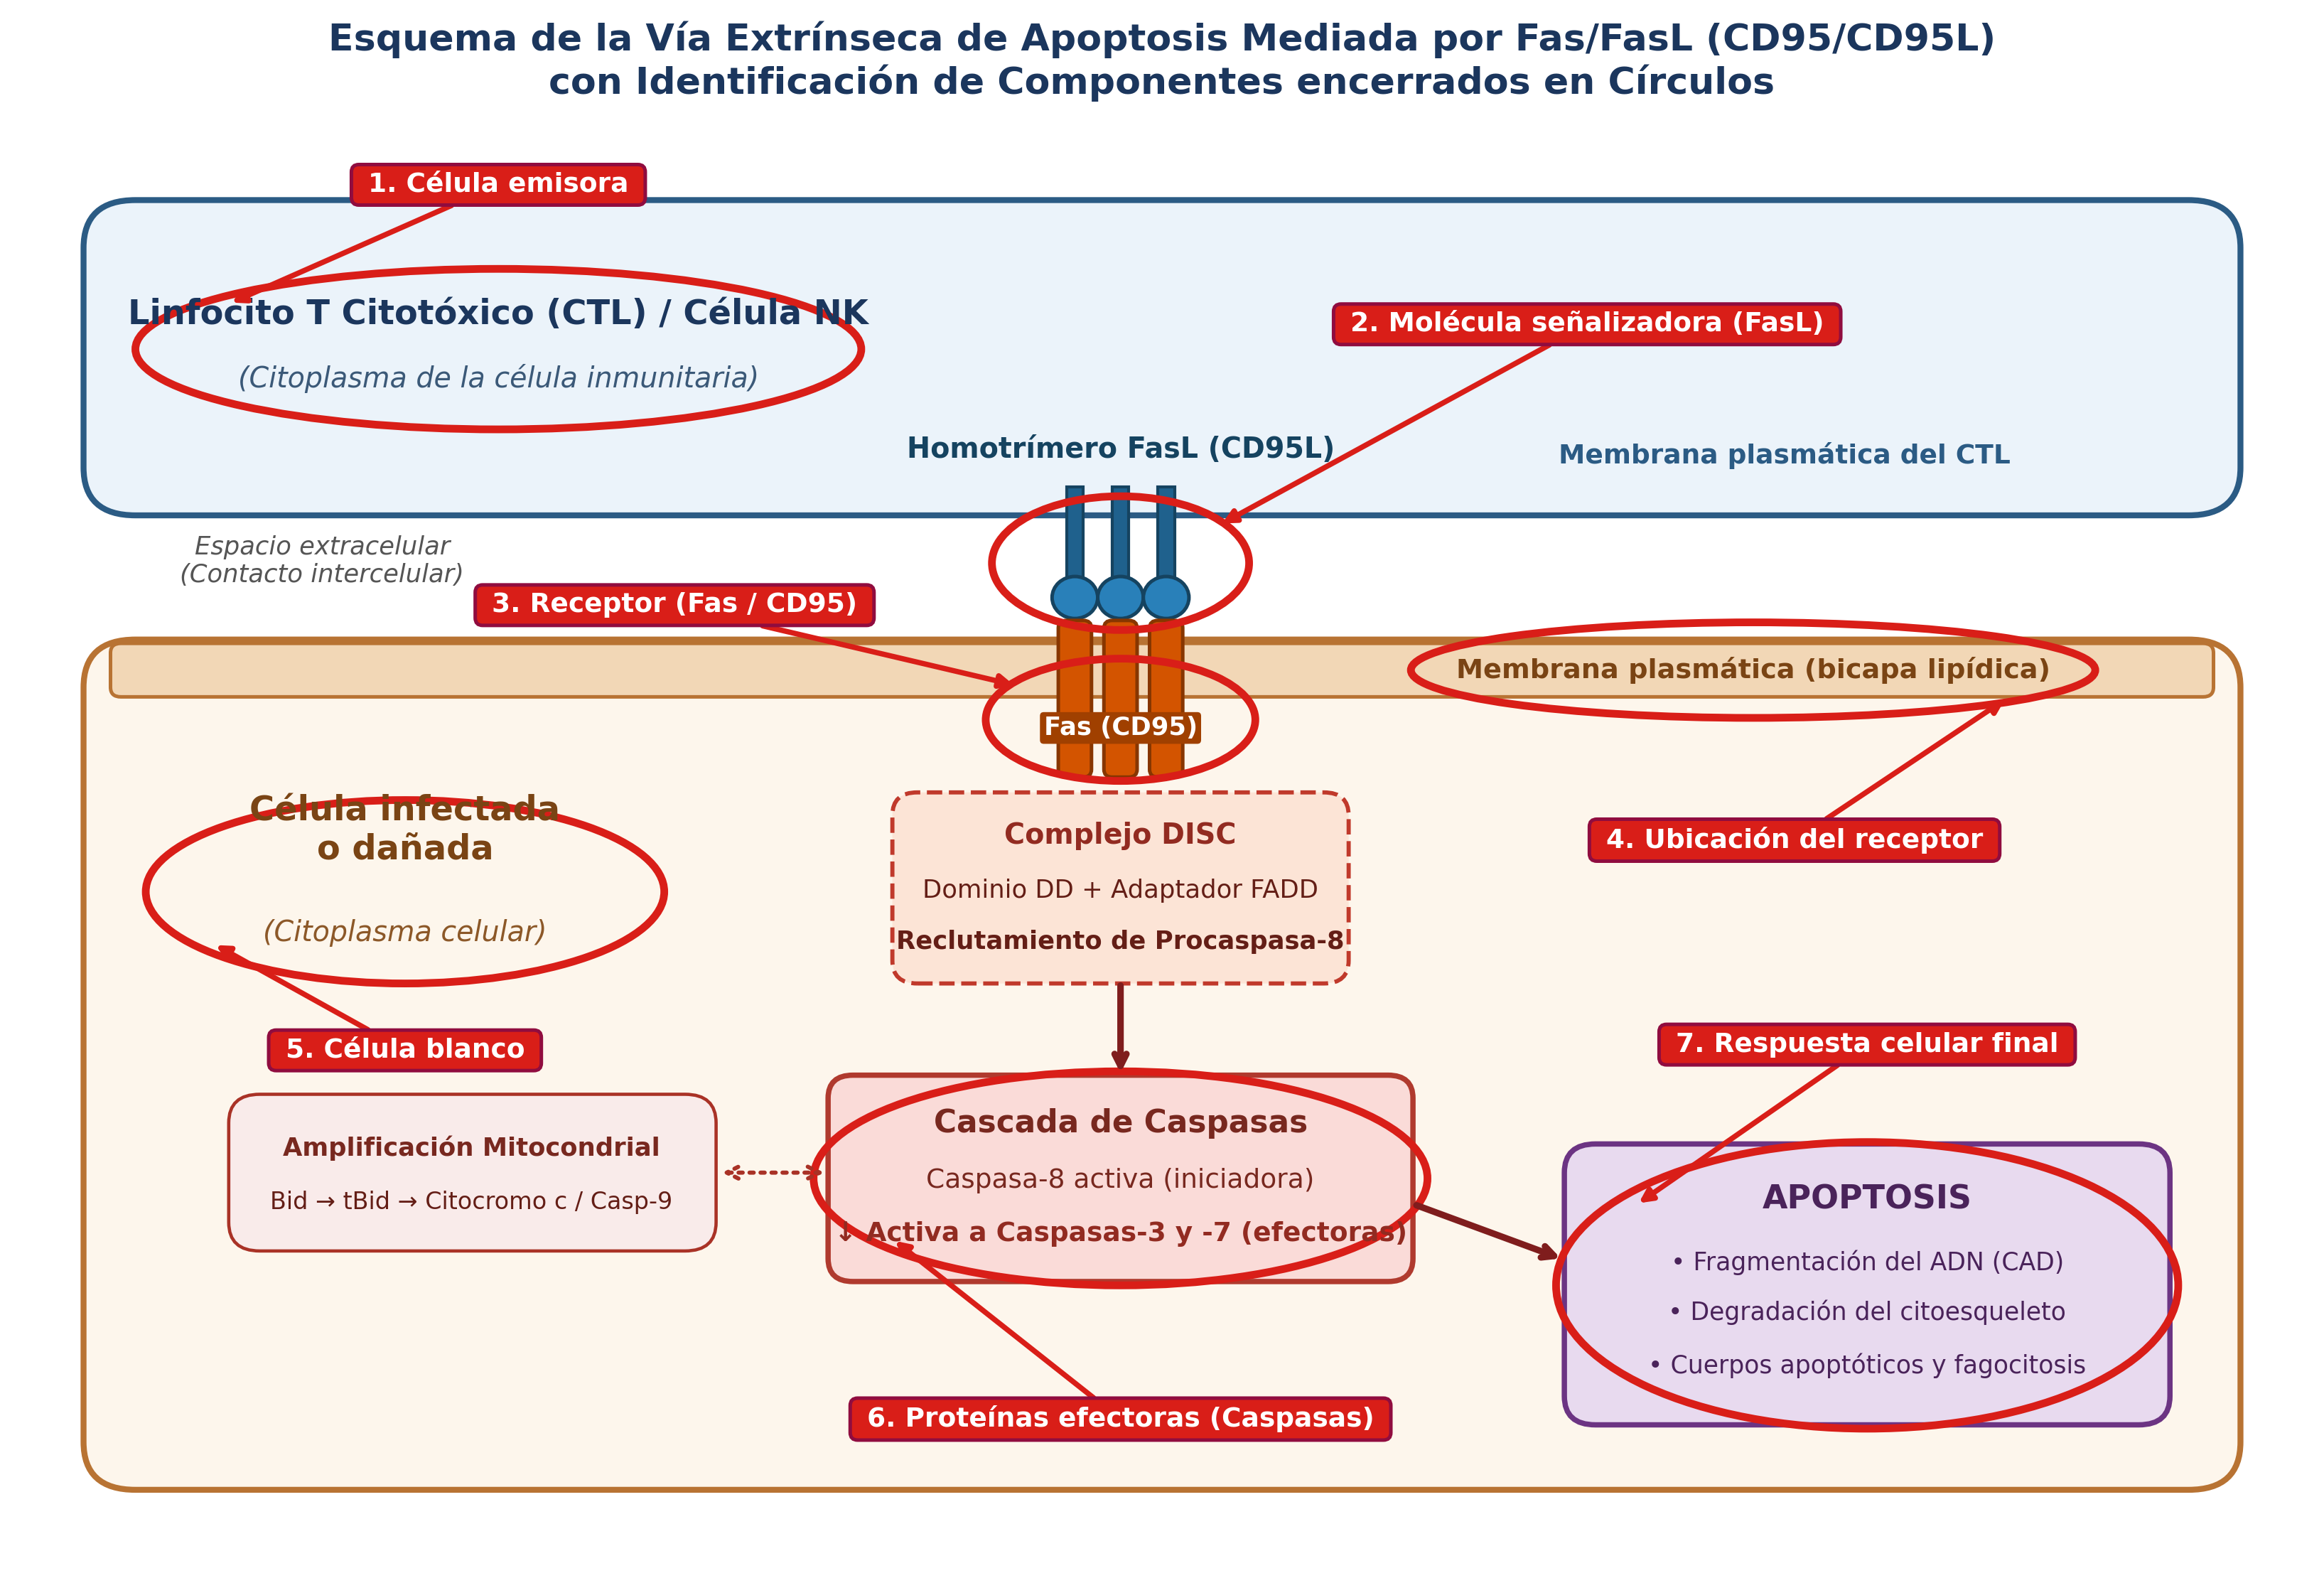
\includegraphics[width=0.88\textwidth,height=0.44\textheight,keepaspectratio]{img/esquema-apoptosis-fas-fasl.png}
	\caption[Esquema integral de la vía apoptótica extrínseca mediada por Fas/FasL]{Esquema integral de la vía de señalización apoptótica extrínseca mediada por Fas/FasL. Los círculos rojos identifican explícitamente los 7 componentes nodales de la vía: \textbf{(1)} Célula emisora (Linfocito T citotóxico / CTL), \textbf{(2)} Molécula señalizadora (FasL), \textbf{(3)} Receptor de muerte de membrana plasmática (Fas / CD95), \textbf{(4)} Célula blanco (célula infectada o dañada), \textbf{(5)} Ubicación del receptor en membrana plasmática y ensamble del DISC, \textbf{(6)} Proteínas efectoras (caspasas iniciadoras y efectoras 8, 3, 6 y 7), y \textbf{(7)} Respuesta celular final (fragmentación apoptótica controlada). Adaptado de \textcite{strasser2009many} y NCBI Bookshelf \parencite{wajant2002fasl}.}
	\label{fig:esquema-fas-fasl}
\end{figure}
\FloatBarrier

\subsection{Correspondencia de los Componentes Identificados}
\begin{itemize}[leftmargin=1.8em,itemsep=0.25em]
	\item \textbf{Círculo 1 --- Célula emisora:} Linfocito T citotóxico (CTL) o célula NK encargada del reconocimiento antigénico y la presentación de ligandos de muerte en su superficie.
	\item \textbf{Círculo 2 --- Molécula señalizadora:} Homotrímero FasL (CD95L), proteína de membrana soluble/anclada que actúa como mensajero químico inductivo.
	\item \textbf{Círculo 3 --- Receptor:} Receptor Fas (CD95 / APO-1), glicoproteína transmembrana con dominio de muerte citoplásmico.
	\item \textbf{Círculo 4 --- Célula blanco:} Célula diana que alberga el daño genotóxico irreversible, infección viral o alteración tisular.
	\item \textbf{Círculo 5 --- Ubicación del receptor y transducción:} Membrana plasmática de la célula blanco, acoplada al complejo DISC mediante la proteína adaptadora citosólica FADD.
	\item \textbf{Círculo 6 --- Proteínas efectoras:} Cascada proteolítica de caspasas iniciadoras (caspasa-8) y caspasas efectoras o ejecutoras (caspasa-3, 6 y 7).
	\item \textbf{Círculo 7 --- Respuesta celular final:} Desmantelamiento y eliminación ordenada de la célula mediante cuerpos apoptóticos reconocidos por macrófagos.
\end{itemize}

\subsection{Matriz de Caracterización de la Vía Celular}
A continuación se presenta la matriz analítica comparativa de las propiedades moleculares y biológicas del eje de señalización examinado, destacando y seleccionando formalmente la opción correspondiente para cada dimensión funcional:

\begin{AulatexTable}[breakable]
\begin{xltabular}{\linewidth}{@{}>{\bfseries\raggedright\arraybackslash\hspace{0pt}}p{4.3cm} >{\raggedright\let\newline\\\arraybackslash\hspace{0pt}}X@{}}
\caption[Matriz comparativa de caracterización funcional del eje Fas/FasL]{Matriz analítica comparativa de las 13 dimensiones moleculares y biológicas del eje de señalización Fas/FasL.}\label{tab:matriz-fas-fasl}\\
\toprule
Elemento & \textbf{Opciones de caracterización (Opción correcta destacada y seleccionada)} \\
\midrule
\endfirsthead
\multicolumn{2}{@{}l}{\small\itshape Continuación de la Tabla \thetable\ --- Matriz analítica del eje Fas/FasL}\\[0.1cm]
\toprule
Elemento & \textbf{Opciones de caracterización (Opción correcta destacada y seleccionada)} \\
\midrule
\endhead
\midrule
\multicolumn{2}{r@{}}{\small\itshape Continúa en la siguiente página\ldots} \\
\endfoot
\bottomrule
\endlastfoot
Tipo de señalización & \selnum{1} \textbf{Paracrina o contacto celular} \optsep Endocrina \optsep Autocrina \\[0.14cm]
Molécula señalizadora & \selnum{1} \textbf{FasL (ligando Fas)} \optsep Insulina \optsep Adrenalina \\[0.14cm]
Naturaleza química & \selnum{1} \textbf{Proteína} \optsep Polisacárido \optsep Lípido \\[0.14cm]
Célula emisora & \selnum{1} \textbf{Linfocito T citotóxico} \optsep Fibroblasto \optsep Hepatocito \\[0.14cm]
Célula blanco & \selnum{1} \textbf{Célula infectada o dañada} \optsep Neurona \optsep Eritrocito \\[0.14cm]
Tipo de receptor & GPCR \optsep \selnum{2} \textbf{Receptor de muerte (Fas/CD95)} \optsep RTK \\[0.14cm]
Ubicación del receptor & Mitocondria \optsep \selnum{2} \textbf{Membrana plasmática} \optsep Núcleo \\[0.14cm]
Clasificación del receptor & Canal iónico \optsep \selnum{2} \textbf{Receptor de membrana} \optsep Receptor intracelular \\[0.14cm]
Transducción de señal & Producción de ATP \optsep \selnum{2} \textbf{Activación de proteínas intracelulares} \optsep Fijación de CO$_2$ \\[0.14cm]
Amplificación de señal & \selnum{1} \textbf{Sí} \optsep Variable \optsep No \\[0.14cm]
Proteínas efectoras principales & Rubisco \optsep \selnum{2} \textbf{Caspasas} \optsep Tubulina \\[0.14cm]
Respuesta celular final & \selnum{1} \textbf{Apoptosis} \optsep Síntesis proteica \optsep Contracción muscular \\[0.14cm]
Resultado biológico & Producción de ATP \optsep \selnum{2} \textbf{Eliminación ordenada de la célula} \optsep División celular \\
\end{xltabular}
\end{AulatexTable}

\subsection{Análisis de Preguntas Fundamentales y Respuestas de Caso}
Con el objetivo de profundizar en la significación biológica de los procesos estudiados, se examinan a continuación cinco cuestiones cardinales sobre la muerte celular programada:

\begin{enumerate}[label=\textbf{\arabic*.}]
	\item \textbf{¿Qué tipo de daño celular puede provocar que una célula entre en apoptosis?}\\
	\textbf{Respuesta:} Diversos tipos de estrés celular agudo e irreversible desencadenan apoptosis, dividiéndose según la vía de señalización implicada:
	\begin{itemize}[leftmargin=1.5em,itemsep=0.15em]
		\item \emph{Vía extrínseca (receptores de muerte):} Infecciones intracelulares virales o bacterianas en las que la célula presenta antígenos extraños en su complejo mayor de histocompatibilidad clase I (MHC-I), induciendo el acoplamiento de FasL expresado por linfocitos T citotóxicos \parencite{caulfield2014disruption}.
		\item \emph{Vía intrínseca (mitocondrial):} Daño severo e irreparable en la doble hebra del ADN causado por radiación ultravioleta, radiación ionizante o agentes quimioterápicos; estrés oxidativo severo por acumulación de especies reactivas de oxígeno (ROS); estrés prolongado del retículo endoplasmático por acumulación masiva de proteínas mal plegadas (UPR no compensada); privación crítica de nutrientes esenciales o pérdida de señales tróficas y factores de crecimiento extracelular indispensables para la supervivencia celular \parencite{strasser2009many,lodish2021molecular}.
	\end{itemize}

	\item \textbf{¿Por qué la apoptosis se considera una muerte celular programada?}\\
	\textbf{Respuesta:} Se define como una muerte celular programada porque no constituye una lisis caótica o pasiva originada por un traumatismo inespecífico, sino la ejecución estricta y secuencial de un programa bioquímico y genético altamente coordinado y dependiente de energía metabólica (ATP). Este programa se encuentra predeterminado en el genoma y opera mediante una cascada proteolítica ordenada de caspasas que degrada selectivamente proteínas del citoesqueleto, láminas nucleares y factores de transcripción, al tiempo que activa endonucleasas que seccionan el genoma en fragmentos internucleosomales precisos sin alterar la permeabilidad primaria de la membrana plasmática ni liberar enzimas hidrolíticas nocivas \parencite{wajant2002fasl,alberts2022molecular}.

	\item \textbf{¿Qué ventaja tiene la apoptosis para un organismo multicelular?}\\
	\textbf{Respuesta:} Ofrece ventajas adaptativas y fisiológicas vitales:
	\begin{itemize}[leftmargin=1.5em,itemsep=0.15em]
		\item \emph{Homeostasis tisular dinámica:} Garantiza un equilibrio exacto entre el ritmo de proliferación celular por mitosis y la eliminación de células envejecidas o redundantes, preservando la masa y arquitectura funcional de los órganos.
		\item \emph{Morfogénesis y desarrollo embrionario:} Permite el modelado estructural de tejidos (por ejemplo, la regresión de las membranas interdigitales para formar dedos libres en vertebrados) y la remodelación de cavidades anatómicas.
		\item \emph{Inmunotolerancia y defensa:} Posibilita la deleción clonal de linfocitos T y B autorreactivos durante la maduración en el timo y médula ósea (previniendo autoinmunidad severa), así como la erradicación segura de células huésped convertidas en reservorio viral, evitando la diseminación del patógeno.
		\item \emph{Ausencia de respuesta inflamatoria nociva:} Al generar cuerpos apoptóticos envueltos en membrana que exponen fosfatidilserina hacia la superficie externa (señal \emph{eat-me}), los fagocitos mononucleares los internalizan sin inducir quimiotaxis proinflamatoria ni colapso de las células circundantes sanas \parencite{caulfield2014disruption,abbas2022cellular}.
	\end{itemize}

	\item \textbf{¿Qué podría ocurrir si una célula con daño grave en su ADN no entrara en apoptosis?}\\
	\textbf{Respuesta:} Si una célula con daño genotóxico irreversible elude el punto de control apoptótico (por ejemplo, por inactivación mutacional de la proteína p53 o hiperactivación de moléculas antiapoptóticas como Bcl-2), continuará completando ciclos de división celular no supervisados. Esto provocará la replicación y transmisión hereditaria de aberraciones cromosómicas, deleciones y mutaciones oncogénicas a todas sus células hijas, lo que conduce a la inestabilidad genómica severa, acumulación de atipias citológicas, inmortalización replicativa y transformación neoplásica hacia tumores malignos (carcinogénesis) \parencite{lodish2021molecular,guegan2022fas}. Asimismo, en el sistema inmunitario puede propiciar la proliferación patológica de clonas autorreactivas e hiperplasia linfoide letal, como ocurre en el síndrome linfoproliferativo autoinmune (ALPS) ocasionado por defectos genéticos en el eje Fas/FasL \parencite{strasser2009many}.

	\item \textbf{¿Qué diferencia general existe entre apoptosis y necrosis?}\\
	\textbf{Respuesta:} La diferencia fundamental radica en el mecanismo termodinámico, morfológico y fisiológico del deceso celular:
	\begin{itemize}[leftmargin=1.5em,itemsep=0.15em]
		\item \textbf{Apoptosis:} Es un proceso fisiológico o de defensa activo, sincronizado y estrictamente dependiente de ATP. Morfológicamente cursa con retracción celular, picnosis (condensación cromatínica), cariorrexis controlada, formación de proyecciones o brotes de membrana (\emph{blebbing}) y fragmentación en cuerpos apoptóticos íntegros. La membrana plasmática conserva su integridad de barrera durante todo el proceso, impidiendo el derrame del citoplasma y culminando en una fagocitosis silenciosa que \textbf{no genera inflamación}.
		\item \textbf{Necrosis:} Es una forma de muerte celular patológica, desregulada y no dependiente de energía celular (pasiva), provocada por agresiones agudas térmicas, isquémicas o toxinas agresivas. Se caracteriza por un fallo osmótico catastrófico con entrada desmedida de agua e iones (oncosis), hinchazón organelar, pérdida prematura de la continuidad de la membrana celular y estallido lítico con liberación masiva de patrones moleculares asociados al daño (DAMPs) y enzimas citoplasmáticas lisosomales al estroma circundante, lo que \textbf{desencadena una potente reacción inflamatoria aguda} y necrosis secundaria de las células tisulares adyacentes \parencite{alberts2022molecular,guegan2022fas}.
	\end{itemize}
\end{enumerate}

\clearpage
\section{Conclusiones Fisiológicas y Perspectiva Agronómica}
La caracterización de la vía de señalización Fas/FasL evidencia que la comunicación celular yuxtacrina no opera exclusivamente como un estímulo trófico o metabólico positivo, sino también como un sofisticado circuito de arbitraje y seguridad biológica capaz de desencadenar la autoliquidación programada cuando una célula pone en peligro la viabilidad global del organismo.

Desde una perspectiva analítica propia, considero que distinguir con precisión biofísica el ligando extracelular, el dominio intracelular de muerte y la cascada proteolítica de caspasas es indispensable para la comprensión integral de la fisiología moderna. El análisis realizado me lleva a sostener que estas conclusiones son directamente transferibles al ámbito de la agronomía y la fitopatología: en el reino vegetal, las respuestas de muerte celular programada análogas (como la reacción de hipersensibilidad o HR) constituyen la barrera primordial que confina las infecciones fúngicas y bacterianas, garantizando la sanidad vegetal y la productividad agrícola sostenible.\footnote{En la elaboración de este trabajo se utilizaron herramientas de inteligencia artificial como apoyo para la organización estructural y revisión de estilo del texto, conforme a los lineamientos de integridad y ética académica institucional. El análisis conceptual, la verificación de fuentes primarias y la postura sostenida son de autoría del estudiante.}

\clearpage
\printbibliography
\end{document}
